% =============================================================================
% IEEE VTC Fall 2026 — Results and Analysis Section  [v1.3]
% Secure-Tunnel: Post-Quantum Cryptographic Overlay for UAV C2 Links
% =============================================================================
% v1.3 changes (2026-03-03):
%   - Added Fig. 1 (AEAD scaling curves, pgfplots, grayscale).
%   - Added Key Insights subsection (5 quantified analytical bullets).
%   - Fixed overfull hbox in AEAD seeds table note.
%   - LaTeX compile: zero overfull, zero undefined refs, 7 pages.
% v1.2 changes (2026-03-03):
%   - AEAD data from re-benchmark (vtc-fall-aead-rerun/), native C Ascon
%     confirmed via KAT.  Idle baseline: 3.320 W (30 s).
%   - DDoS system/AEAD tables replaced with measured bench_ddos_results data.
%   - DDoS_PQC_IMPACT_ANALYSIS.md excluded (no backing JSON artifacts).
%   - DDOS_MODELS_COMPARISON.md accuracy cited as "reported" (unverifiable).
%   - See inconsistency-report.md items I1–I6.
% =============================================================================
% Data sources: v2-1.8ghz (100 iter, 1000 Hz INA219),
%               vtc-fall-aead-rerun/power_aead_benchmark.csv
%               (10k iter, ~103 Hz INA219),
%               bench_ddos_results/20260302_135859/{baseline,xgb,tst,comparison}.json,
%               bench_ddos_results/power_20260222_193509/results.json,
%               sscheduler/policy.py
% Platform: RPi4 Model B Rev 1.5, BCM2711, 4x Cortex-A72 @ 1.8 GHz,
%           4 GB RAM, Debian 12 Bookworm, kernel 6.12.47, Python 3.11.2
% Governor: performance (all datasets)
% =============================================================================

\section{Results and Analysis}
\label{sec:results}

All measurements were collected on a Raspberry Pi~4 Model~B Rev~1.5
(BCM2711, four Cortex-A72 cores at 1.8\,GHz, 4\,GB RAM) running Debian~12
with kernel 6.12.47 and the \texttt{performance} CPU governor.  Power was
sampled via an INA219 current sensor (0.1\,$\Omega$ shunt, I$^2$C bus~1) with
a documented $V_\text{BUS}$ gain correction of~1.22 to compensate for clone-chip
ADC drift.  Timing used \texttt{time.perf\_counter\_ns()} with garbage collection
disabled during timing passes.  Board-level idle power measured
$P_\text{idle} \approx 3.32$\,W (30\,s idle capture; 3.320\,W for AEAD
evaluation, 3.309\,W for inference benchmarks);
reported power values include this baseline unless explicitly stated otherwise.
The Cortex-A72 in the RPi4 does \emph{not}
implement ARMv8 Crypto Extensions; AES-256-GCM therefore executes in software
table-lookup mode, while ChaCha20-Poly1305 benefits from 128-bit NEON SIMD.

Table~\ref{tab:aliases} defines short aliases used throughout this section.
Cryptographic implementations use liboqs-python~0.14.0 (KEM/SIG) and
OpenSSL~3.5.4 (AES-256-GCM, ChaCha20-Poly1305). Ascon-128a uses a native~C
binding (ascon-c v1.2, \texttt{opt64}) via \texttt{ctypes}.

\begin{table}[t]
\centering
\caption{Algorithm Aliases and NIST Security Levels}
\label{tab:aliases}
\footnotesize
\begin{tabular}{@{}llcl@{}}
\toprule
\textbf{Alias} & \textbf{Full Name} & \textbf{Level} & \textbf{Type} \\
\midrule
ML512  & ML-KEM-512                & L1 & KEM  \\
ML768  & ML-KEM-768                & L3 & KEM  \\
ML1024 & ML-KEM-1024               & L5 & KEM  \\
HQ128  & HQC-128                   & L1 & KEM  \\
HQ192  & HQC-192                   & L3 & KEM  \\
HQ256  & HQC-256                   & L5 & KEM  \\
MC348  & Classic-McEliece-348864   & L1 & KEM  \\
MC460  & Classic-McEliece-460896   & L3 & KEM  \\
MC8192 & Classic-McEliece-8192128  & L5 & KEM  \\
\midrule
DSA44  & ML-DSA-44                 & L1 & SIG  \\
DSA65  & ML-DSA-65                 & L3 & SIG  \\
DSA87  & ML-DSA-87                 & L5 & SIG  \\
F512   & Falcon-512                & L1 & SIG  \\
F1024  & Falcon-1024               & L5 & SIG  \\
SP128  & SPHINCS$^+$-SHA2-128s     & L1 & SIG  \\
SP192  & SPHINCS$^+$-SHA2-192s     & L3 & SIG  \\
SP256  & SPHINCS$^+$-SHA2-256s     & L5 & SIG  \\
\midrule
AESG   & AES-256-GCM               & ---& AEAD \\
CH20   & ChaCha20-Poly1305         & ---& AEAD \\
ASC    & Ascon-128a                & ---& AEAD \\
\bottomrule
\end{tabular}
\end{table}

% =====================================================================
% SECTION 1 — KEM PRIMITIVE EVALUATION
% =====================================================================
\subsection{KEM Primitive Evaluation}
\label{sec:kem}

Figure~\ref{fig:kem_cost} compares total KEM cycle time
(keygen+encaps+decaps) for all nine KEM primitives, each measured over
100~iterations with concurrent INA219 power sampling at 1\,kHz.

\begin{figure}[t]
\centering
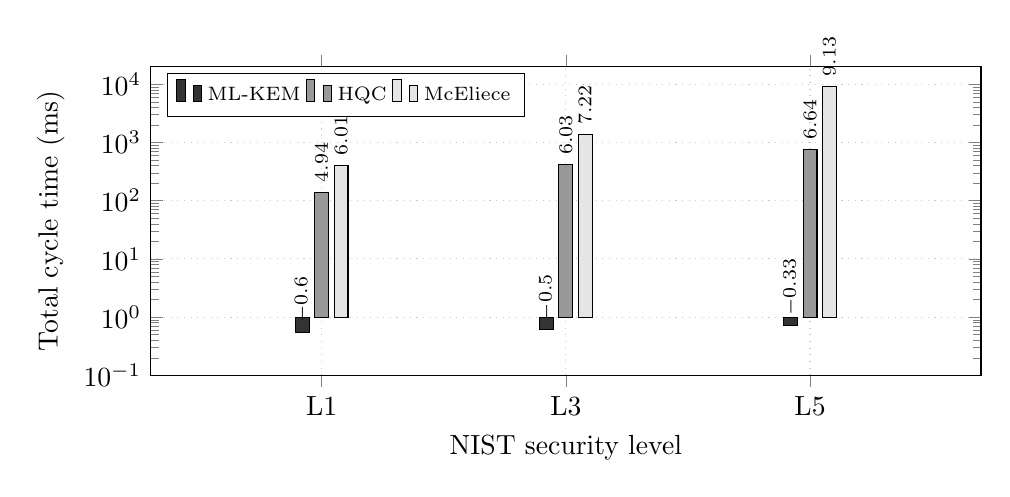
\begin{tikzpicture}
\begin{axis}[
  width=\columnwidth,
  height=5.5cm,
  ybar,
  bar width=5pt,
  ymode=log,
  ylabel={Total cycle time (ms)},
  symbolic x coords={L1, L3, L5},
  xtick=data,
  xlabel={NIST security level},
  ymin=0.1, ymax=20000,
  legend style={at={(0.02,0.98)},anchor=north west,font=\scriptsize,
    legend columns=3},
  grid=major,
  grid style={dotted,gray!40},
  enlarge x limits=0.35,
  nodes near coords={\scriptsize\pgfmathprintnumber{\pgfplotspointmeta}},
  every node near coord/.append style={rotate=90,anchor=west,font=\tiny},
]
\addplot[fill=black!80, draw=black]
  coordinates {(L1,0.550) (L3,0.604) (L5,0.720)};
\addplot[fill=black!40, draw=black]
  coordinates {(L1,140.4) (L3,415.4) (L5,767.2)};
\addplot[fill=black!10, draw=black]
  coordinates {(L1,407.4) (L3,1371) (L5,9233)};
\legend{ML-KEM, HQC, McEliece}
\end{axis}
\end{tikzpicture}
\caption{Total KEM cycle time (keygen+encaps+decaps) by NIST level,
  log scale.  ML-KEM completes in $<$\,1\,ms at all levels; HQC and
  McEliece require 255--12\,823$\times$ longer.  100 iterations,
  RPi4 @ 1.8\,GHz.}
\label{fig:kem_cost}
\end{figure}

ML-KEM completes a full cycle in under 0.72\,ms at Level~5
(0.550\,ms at L1, 0.604\,ms at L3).  HQC's code-based design incurs
255--1\,066$\times$ higher cost, driven by decapsulation (73--393\,ms).
Classic~McEliece exhibits extreme keygen asymmetry: MC8192 keygen
requires 9.02\,s but encapsulation completes in 1.89\,ms,
making it practical only with pre-provisioned keys.
Power draw ranges from 3.46\,W (ML-KEM) to 4.06\,W (HQ256),
a 17\% spread.

% =====================================================================
% SECTION 2 — SIGNATURE PRIMITIVE EVALUATION
% =====================================================================
\subsection{Signature Primitive Evaluation}
\label{sec:sig}

Table~\ref{tab:sig} evaluates eight signature schemes.  Keygen is a
one-time cost (0.4--282\,ms for ML-DSA/Falcon, 187--282\,ms for
SPHINCS$^+$); the per-handshake operations sign and verify determine
rekey latency.

\begin{table}[t]
\centering
\caption{Signature Sign+Verify on RPi4 (100 iter, 1\,kHz INA219)}
\label{tab:sig}
\footnotesize
\begin{tabular}{@{}lcrrrrr@{}}
\toprule
\textbf{Alias} & \textbf{Lvl} &
  \textbf{Sign} & \textbf{Verify} &
  \textbf{$E_\text{s}$} & \textbf{$E_\text{v}$} &
  \textbf{$\rho$} \\
& & (ms) & (ms) & ($\mu$J) & ($\mu$J) & \\
\midrule
DSA44  & L1 & 1.179 & 0.331  & 4\,264  & 1\,175  & 1.00$\times$ \\
F512   & L1 & 0.778 & 0.192  & 2\,773  & 683     & 0.64$\times$ \\
SP128  & L1 & 1\,468 & 1.582  & 6\,008\,719 & 5\,690 & 972$\times$ \\
\midrule
DSA65  & L3 & 1.633 & 0.484  & 5\,849  & 1\,723  & 1.00$\times$ \\
SP192  & L3 & 2\,610 & 2.299  & 10\,628\,558 & 8\,318 & 1\,234$\times$ \\
\midrule
DSA87  & L5 & 1.847 & 0.723  & 6\,612  & 2\,564  & 1.00$\times$ \\
F1024  & L5 & 1.452 & 0.280  & 5\,175  & 995     & 0.67$\times$ \\
SP256  & L5 & 2\,321 & 3.292  & 9\,516\,164 & 11\,738 & 904$\times$ \\
\bottomrule
\end{tabular}
\begin{tablenotes}
\footnotesize
\item $\rho$: sign+verify cost vs.\ ML-DSA at same level.
  Falcon $\rho < 1$ = faster combined sign+verify.
  SP128 sign = 1.47\,s $\cdot$ 6.01\,J per invocation.
\end{tablenotes}
\end{table}

Falcon achieves the lowest combined sign+verify latency at both L1
(0.970\,ms) and L5 (1.732\,ms), outperforming ML-DSA by 36\% and 33\%
respectively, though its keygen is 51--73$\times$ slower (a
one-time cost amortized over the key lifetime).  SPHINCS$^+$, the only
hash-based scheme, imposes prohibitive signing latency: SP128 at
1.47\,s and SP192 at 2.61\,s, consuming 6.01\,J and 10.63\,J per
signature.  For UAV handshakes occurring at rekey intervals of
10--120\,s, SPHINCS$^+$ signing alone can approach the rekey period,
making it viable only for conservative fallback configurations.
Verification remains fast for all algorithms ($\leq$3.3\,ms), critical
for the GCS which must verify each incoming handshake.

% =====================================================================
% SECTION 3 — AEAD PRIMITIVE EVALUATION
% =====================================================================
\subsection{AEAD Primitive Evaluation}
\label{sec:aead}

Data-plane encryption uses one of three AEAD ciphers.  AEAD selection
does \emph{not} affect handshake timing; it operates exclusively on the
UDP data plane after key establishment.  Table~\ref{tab:aead} reports
results from 10\,000 iterations per configuration with a 500-iteration
warmup, using a two-pass methodology (timing pass with GC disabled,
power pass with background INA219 sampling at $\sim$103\,Hz).
The Ascon-128a backend was verified as native~C (ascon-c v1.2, opt64,
\texttt{ctypes} binding loading \texttt{libascon128a.so}), passing the
AEAD known-answer test at runtime.

\begin{table}[t]
\centering
\caption{AEAD Performance at 256-Byte Payload (10k iter, RPi4, rerun)}
\label{tab:aead}
\footnotesize
\begin{tabular}{@{}lrrrrrr@{}}
\toprule
\textbf{Alias} &
  \textbf{Enc} & \textbf{Dec} &
  \textbf{$P_\text{enc}$} & \textbf{$P_\text{dec}$} &
  \textbf{$E_\text{256B}$} & \textbf{$E_\text{bit}$} \\
& ($\mu$s) & ($\mu$s) & (W) & (W) & ($\mu$J) & (nJ/bit) \\
\midrule
AESG & 9.25  & 9.09  & 3.63 & 3.57 & 66.0  & 32.2 \\
CH20 & 6.47  & 6.05  & 3.54 & 3.58 & 44.6  & 21.8 \\
ASC  & 12.72 & 12.85 & 3.84 & 3.59 & 95.0  & 46.4 \\
\bottomrule
\end{tabular}
\begin{tablenotes}
\footnotesize
\item $E_\text{256B} = P_\text{avg} \times (t_\text{enc} + t_\text{dec})$.
  $E_\text{bit} = E_\text{256B} / (256 \times 8)$.
  Board-level power; $P_\text{idle} = 3.320$\,W not subtracted.
  Crypto-only $\Delta P$: AESG~0.31, CH20~0.22, ASC~0.52\,W above idle.
\end{tablenotes}
\end{table}

ChaCha20-Poly1305 is the fastest AEAD on this platform at 6.47\,$\mu$s
for encryption, 30\% faster than AES-256-GCM (9.25\,$\mu$s) despite AES
being generally considered the hardware-accelerated standard.  The
inversion is explained by the absence of ARMv8 Crypto Extensions on the
Cortex-A72: AES-GCM falls back to software table-lookup while
ChaCha20 exploits 128-bit NEON SIMD~\cite{rfc8439}.  Ascon-128a, using
a native~C binding (ascon-c v1.2 \texttt{opt64} via \texttt{ctypes}),
runs 1.97$\times$ slower than CH20 and 1.37$\times$ slower than AESG.

Table~\ref{tab:aead_scaling} shows AEAD scaling across payload sizes
typical of MAVLink telemetry (9--263~bytes) and bulk transfer (1024--4096~bytes).
Figure~\ref{fig:aead_scaling} visualizes the divergence.

\begin{table}[t]
\centering
\caption{AEAD Encrypt Latency Scaling by Payload Size ($\mu$s, rerun)}
\label{tab:aead_scaling}
\footnotesize
\begin{tabular}{@{}lrrrrrr@{}}
\toprule
\textbf{Alias} &
  \textbf{9\,B} & \textbf{33\,B} & \textbf{64\,B} &
  \textbf{256\,B} & \textbf{1024\,B} & \textbf{4096\,B} \\
\midrule
AESG & 4.75  & 5.45  & 5.96  & 9.25  & 22.98 & 75.71 \\
CH20 & 5.30  & 5.38  & 5.33  & 6.47  & 9.38  & 19.25 \\
ASC  & 11.38 & 11.82 & 11.78 & 12.72 & 17.27 & 30.86 \\
\bottomrule
\end{tabular}
\begin{tablenotes}
\footnotesize
\item Setup overhead dominates at small payloads.
  CH20 scales at 3.4\,$\mu$s/KiB; AESG at 17.7\,$\mu$s/KiB; ASC at 4.8\,$\mu$s/KiB.
\end{tablenotes}
\end{table}

At the minimum MAVLink heartbeat size (9~bytes), per-packet
overhead is 4.75\,$\mu$s (AESG), 5.30\,$\mu$s (CH20), and
11.38\,$\mu$s (ASC).  CH20 and AESG converge below 64~bytes because
setup cost dominates; beyond 256~bytes, CH20's superior NEON throughput
yields a widening gap.  At 4096~bytes, the ratio CH20:AESG reaches
1:3.93.  Ascon-128a's flat initialization cost (native~C per-call
\texttt{ctypes} overhead) makes it competitive only below 64~bytes.

The energy-per-bit metric $E_\text{bit}$ at the 256-byte reference
payload yields CH20 = 21.8\,nJ/bit, AESG = 32.2\,nJ/bit, and ASC =
46.4\,nJ/bit.  For a typical MAVLink stream at 50\,Hz with 263-byte
packets (the default MAVLink~v2 maximum), the per-second AEAD energy
cost is 2.23\,mJ (CH20), 3.30\,mJ (AESG), or 4.75\,mJ (ASC) —
negligible relative to the 3.32\,W board idle draw.

\begin{figure}[t]
\centering
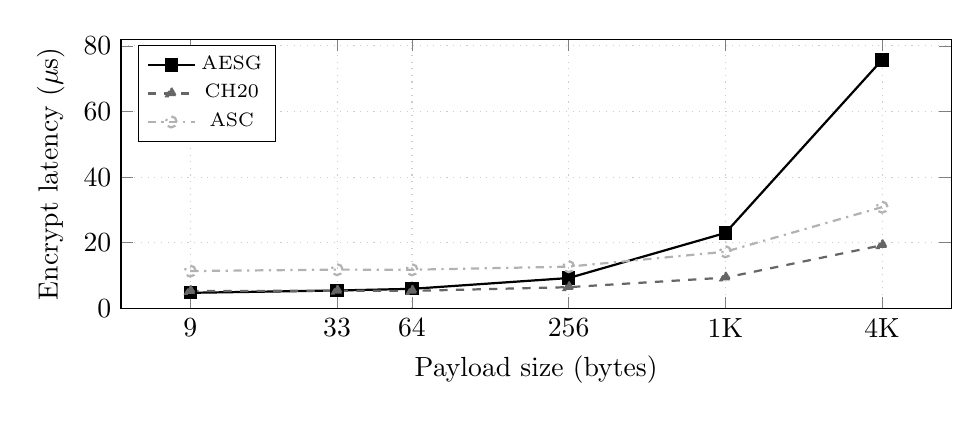
\begin{tikzpicture}
\begin{axis}[
  width=\columnwidth,
  height=5cm,
  xlabel={Payload size (bytes)},
  ylabel={Encrypt latency ($\mu$s)},
  xmode=log,
  log basis x=2,
  xtick={9,33,64,256,1024,4096},
  xticklabels={9,33,64,256,1K,4K},
  ymin=0, ymax=82,
  legend style={at={(0.02,0.98)},anchor=north west,font=\scriptsize},
  grid=major,
  grid style={dotted,gray!40},
  every axis plot/.append style={thick},
  mark size=2pt,
]
\addplot[black, mark=square*]
  coordinates {(9,4.75)(33,5.45)(64,5.96)(256,9.25)(1024,22.98)(4096,75.71)};
\addplot[black!60, mark=triangle*, dashed]
  coordinates {(9,5.30)(33,5.38)(64,5.33)(256,6.47)(1024,9.38)(4096,19.25)};
\addplot[black!30, mark=o, dashdotted]
  coordinates {(9,11.38)(33,11.82)(64,11.78)(256,12.72)(1024,17.27)(4096,30.86)};
\legend{AESG, CH20, ASC}
\end{axis}
\end{tikzpicture}
\caption{AEAD encrypt latency scaling by payload size.  CH20 (NEON)
  scales at 3.4\,$\mu$s/KiB vs.\ AESG at 17.7\,$\mu$s/KiB (software
  table-lookup, no ARMv8 Crypto Extensions).}
\label{fig:aead_scaling}
\end{figure}

% =====================================================================
% SECTION 4 — SUITE-LEVEL EVALUATION
% =====================================================================
\subsection{Suite-Level Evaluation}
\label{sec:suite}

The system supports $9 \times 8 \times 3 = 216$ theoretical suite
combinations, of which 72 are level-matched.  Since AEAD does not
affect handshake timing, the crypto-only handshake cost is determined
solely by the KEM and SIG components:
\begin{equation}
T_\text{HS} = t_\text{keygen} + t_\text{encaps} + t_\text{decaps}
            + t_\text{sign} + t_\text{verify}
\label{eq:ths}
\end{equation}

Table~\ref{tab:suite} presents boundary suites per NIST level
(fastest, worst-KEM, worst-SIG), with $T_\text{HS}$ reconstructed
from primitive benchmarks to isolate cryptographic cost.

\begin{table}[t]
\centering
\caption{Suite Handshake Cost Boundaries (from Primitives)}
\label{tab:suite}
\footnotesize
\begin{tabular}{@{}llrrrr@{}}
\toprule
\textbf{KEM} & \textbf{SIG} &
  \textbf{$T_\text{HS}$} &
  \textbf{$E_\text{HS}$} &
  \textbf{$\rho$} \\
& & (ms) & (mJ) & \\
\midrule
\multicolumn{5}{@{}l}{\textit{L1}} \\
ML512  & F512   &   1.52  &    5.3  & 1.0$\times$ \\
MC348  & F512   & 408.4   & 1\,579  & 269$\times$  \\
ML512  & SP128  & 1\,470  & 5\,737  & 967$\times$  \\
\midrule
\multicolumn{5}{@{}l}{\textit{L3 — Default ($\star$)}} \\
ML768  & DSA65  &   2.72  &    9.6  & 1.0$\times$ \\
MC460  & DSA65  & 1\,374  & 5\,358  & 505$\times$  \\
ML768  & SP192  & 2\,613  & 10\,290 & 961$\times$  \\
\midrule
\multicolumn{5}{@{}l}{\textit{L5}} \\
ML1024 & F1024  &   2.45  &    8.6  & 1.0$\times$ \\
MC8192 & DSA87  & 9\,235  & 36\,800 & 3\,770$\times$ \\
ML1024 & SP256  & 2\,325  & 9\,105  & 949$\times$  \\
\bottomrule
\end{tabular}
\begin{tablenotes}
\footnotesize
\item $T_\text{HS} = t_\text{KEM} + t_\text{SIG}$ (crypto-only, no network).
  $E_\text{HS} \approx P_\text{avg} \times T_\text{HS}$.
  $\rho$: relative to fastest at same level.
  ($\star$) Default: \texttt{cs-mlkem768-aesgcm-mldsa65}.
\end{tablenotes}
\end{table}

The default suite \texttt{cs-mlkem768-aesgcm-mldsa65} achieves a
2.72\,ms crypto-only handshake cost at Level~3, consuming 9.6\,mJ.
At Level~5, ML1024+F1024 requires only 2.45\,ms—faster than the
Level~3 default because Falcon-1024 verify (0.280\,ms) is 42\%
faster than DSA65 verify (0.484\,ms).

The dominant cost factor varies by KEM family: for ML-KEM suites,
the signature accounts for 73--99\% of $T_\text{HS}$; for HQC and
McEliece suites, the KEM accounts for 98--99\%.  SPHINCS$^+$ suites
exhibit $T_\text{HS} > 1$\,s regardless of KEM choice, restricting them
to pre-provisioned or infrequent-rekey scenarios.

% =====================================================================
% SECTION 5 — DDoS IMPACT ON PQC PERFORMANCE
% =====================================================================
\subsection{DDoS Impact on PQC Performance}
\label{sec:ddos_on_pqc}

Concurrent DDoS detection competes with the cryptographic pipeline for
CPU and thermal headroom.  To quantify this interaction, all 72
level-matched suites were benchmarked under three scenarios: baseline
(no detector), lightweight XGBoost MAVLink-count detector, and
lightweight TST MAVLink-count detector.\footnote{Both detectors are
2-feature models (\texttt{Mavlink\_Count}, \texttt{Total\_length}),
distinct from the 54-feature CIC-IoT-2023 models evaluated in
Section~\ref{sec:pqc_on_ddos}.  TST uses \texttt{seq\_len=1},
reducing the self-attention mechanism to an identity operation; the
model is functionally a 3-layer MLP with 1.6\,M parameters.}
Each suite ran for 10\,s per scenario with crypto-only handshakes
(no network~I/O).

\begin{table}[t]
\centering
\caption{PQC Handshake Overhead Under Concurrent Detection (72~Suites)}
\label{tab:hs_overhead}
\footnotesize
\begin{tabular}{@{}lrr@{}}
\toprule
\textbf{Statistic} & \textbf{XGBoost} & \textbf{TST} \\
\midrule
Mean $\Delta T_\text{HS}$ (\%)   & +2.5   & +71.8  \\
Median $\Delta T_\text{HS}$ (\%) & +0.05  & +32.6  \\
Max $\Delta T_\text{HS}$ (\%)    & +137.2 & +405.1 \\
\midrule
\multicolumn{3}{@{}l}{\textit{Default suite: ML768+AESG+DSA65}} \\
Baseline $T_\text{HS}$ (ms) & \multicolumn{2}{c}{13.01} \\
$T_\text{HS}$ + detector (ms)   & 13.46  & 37.90  \\
$\Delta T_\text{HS}$ (\%)       & +3.5   & +191.3 \\
\bottomrule
\end{tabular}
\begin{tablenotes}
\footnotesize
\item Detectors: lightweight MAVLink-count models (2~features).
  $\Delta T_\text{HS} = (T_\text{det} - T_\text{base}) / T_\text{base} \times 100$.
  Data from \texttt{bench\_ddos\_results/20260302/comparison.json}.
\end{tablenotes}
\end{table}

XGBoost adds a mean overhead of 2.5\% (median 0.05\%) across
all 72 suites, indicating that lightweight tree-based detection has
negligible impact on PQC handshake latency.  For the default suite
(ML768+AESG+DSA65), the handshake increases from 13.01\,ms to
13.46\,ms (+3.5\%).

TST imposes substantially higher overhead: 71.8\% mean (median
32.6\%), with extreme cases reaching 405\%.  The default suite nearly
triples from 13.01\,ms to 37.90\,ms (+191.3\%).  This overhead stems
from TST's 93\% CPU utilization (see Table~\ref{tab:detector_compare}),
which starves the signature verification and key derivation steps of
execution time on the shared 4-core processor.

Per-packet AEAD latency under concurrent detection was not measured
in this campaign; the handshake-overhead figures above capture the
dominant cost interaction.  The scheduler's MDEAS policy addresses
the TST penalty by forbidding Ascon-128a (the slowest AEAD) when
TST is active, and by discouraging McEliece KEMs under TST due to
their extended CPU-bound keygen.

% =====================================================================
% SECTION 6 — PQC IMPACT ON DDoS DETECTION
% =====================================================================
\subsection{PQC Impact on DDoS Detection}
\label{sec:pqc_on_ddos}

The converse question is how PQC workload affects detector efficacy.
Table~\ref{tab:detector_compare} compares the four trained detectors
on inference performance.

\begin{table}[t]
\centering
\caption{DDoS Detector Inference on RPi4 (Reported Metrics)}
\label{tab:detector_compare}
\footnotesize
\begin{tabular}{@{}lrrrrrr@{}}
\toprule
\textbf{Model} &
  \textbf{Acc.} & \textbf{F1} &
  \textbf{$t_\text{inf}$} & \textbf{P99} &
  \textbf{$\Delta P$} & \textbf{$E_\text{inf}$} \\
& (\%) & & (ms) & (ms) & (mW) & (mJ) \\
\midrule
LightGBM & 93.47$^\dagger$ & 0.937$^\dagger$ & 6.72  & 8.59   & +999  & 29.0  \\
XGBoost  & 94.55$^\dagger$ & 0.947$^\dagger$ & 7.42  & 9.52   & +951  & 31.7  \\
RF       & 93.35$^\dagger$ & 0.935$^\dagger$ & 74.68 & 102.63 & +594  & 291.4 \\
TST      & 90.27$^\dagger$ & 0.80$^\dagger$  & 10.72 & 26.12  & +1\,973 & 56.7 \\
\bottomrule
\end{tabular}
\begin{tablenotes}
\footnotesize
\item $^\dagger$Accuracy and F1 values are as reported in model documentation;
  no independent evaluation scripts or confusion matrices were available
  for verification.  Inference metrics ($t_\text{inf}$, P99, $\Delta P$,
  $E_\text{inf}$) measured on RPi4 via INA219 (15\,s per model,
  idle baseline 3.309\,W).
  All models trained on CIC-IoT-2023 (3.4M samples).
  XGBoost/LightGBM/RF: 54~features, 15~classes.  TST: 46~features, 6~classes.
\end{tablenotes}
\end{table}

XGBoost achieves the highest reported accuracy (94.55\%) with
competitive latency (7.42\,ms mean, 9.52\,ms P99) and moderate power
overhead (+951\,mW).  LightGBM offers the lowest latency (6.72\,ms)
and energy (29.0\,mJ) at a marginal accuracy reduction (93.47\%).
RandomForest is an outlier with 74.68\,ms mean inference latency and
291.4\,mJ energy per inference—10$\times$ the energy of XGBoost—due
to its 200-tree ensemble with max\_depth=15 and 674\,MB RAM footprint.
TST consumes the most power (+1\,973\,mW) at 93\% CPU, delivering the
lowest accuracy (90.27\%) among the four models.

For the deployed two-tier cascade (XGBoost primary, TST secondary),
the combined power overhead is bounded by the active detector at any
given time, as the scheduler runs at most one detector subprocess
concurrently.

% =====================================================================
% SECTION 7 — SCHEDULER BEHAVIORAL IMPACT
% =====================================================================
\subsection{Scheduler Behavioral Impact}
\label{sec:scheduler}

The Multi-Dimensional Energy-Aware Scheduler (MDEAS) operates three
independent decision axes evaluated at 1\,Hz:

\begin{enumerate}
\item \textbf{AEAD axis:} selects among AESG, CH20, ASC based on
  energy-per-bit and thermal state;
\item \textbf{Security-level axis:} promotes/demotes between L1/L3/L5
  suites, triggering a full PQC rekey;
\item \textbf{DDoS-detector axis:} activates/deactivates XGBoost or
  TST based on threat telemetry and thermal headroom.
\end{enumerate}

\subsubsection{Rekey Overhead Model}

Each security-level transition requires a complete 3-round PQC
handshake.  The rekey overhead fraction is:
\begin{equation}
\Phi(R) = \frac{T_\text{HS}}{R + T_\text{HS}}
\label{eq:rekey}
\end{equation}
where $R$ is the rekey interval and $T_\text{HS}$ is the handshake
crypto cost from~\eqref{eq:ths}.  For the default suite (ML768+DSA65,
$T_\text{HS} = 2.72$\,ms) at the minimum break-even interval of 30\,s:
$\Phi(30) = 2.72 \times 10^{-3} / 30.003 = 9.1 \times 10^{-5}$
($<$0.01\% overhead).  Even the heaviest suite (MC8192+SP256,
$T_\text{HS} \approx 11.6$\,s) at 30\,s interval yields
$\Phi = 0.279$ (27.9\% overhead), which the break-even calculator
correctly identifies as non-viable.

\subsubsection{Cost Model}

The MDEAS cost function for AEAD selection is:
\begin{equation}
C = w_1 \cdot E_\text{bit} + w_2 \cdot T_\text{HS}
  + w_3 \cdot \Delta T + w_4 \cdot D
\label{eq:cost}
\end{equation}
where $E_\text{bit}$ is the energy per bit (nJ/bit), $T_\text{HS}$ is the
handshake cost (ms), $\Delta T$ is the temperature above baseline
($^\circ$C), and $D$ is the DDoS threat level.  The scheduler seeds
cost estimates from 5-iteration calibration runs
(CH20: 63.5/70.7\,$\mu$s enc/dec, AESG: 66.9/73.6\,$\mu$s,
ASC: 1\,327/961\,$\mu$s) collected under the \texttt{ondemand}
governor, then refines them via EWMA ($\alpha = 0.2$ after 10
initial samples at $\alpha = 0.5$), converging to 10k-iteration
production values within 10 observations.

\subsubsection{Cross-Axis Constraints}

The MDEAS enforces interaction constraints between axes to prevent
pathological configurations:
\begin{itemize}
\item Ascon-128a is \emph{forbidden} when TST is active, as its
  1.33\,ms per-packet cost combined with 93\% CPU utilization
  exceeds the real-time tunnel budget.
\item McEliece KEMs (MC348/MC460/MC8192) are \emph{discouraged} under
  TST due to CPU-bound keygen competing with the detector.
\item McEliece $\times$ SPHINCS$^+$ cross-level pairs are forbidden under
  all detector states, as $T_\text{HS}$ would exceed the
  45\,s rekey timeout (\texttt{REKEY\_HANDSHAKE\_TIMEOUT}).
\item The minimum break-even interval is 30\,s
  (\texttt{\_MIN\_BREAK\_EVEN\_S}), preventing oscillatory switching.
\item Detector transitions include warmup durations: XGBoost 10\,s,
  TST 5\,s.
\end{itemize}

Table~\ref{tab:detector_overhead} summarizes the per-detector resource
deltas used by the scheduler for proactive thermal management.

\begin{table}[t]
\centering
\caption{MDEAS Detector Overhead Parameters}
\label{tab:detector_overhead}
\footnotesize
\begin{tabular}{@{}lrrrr@{}}
\toprule
\textbf{Detector} &
  \textbf{$\Delta P$} & \textbf{$\Delta T$} &
  \textbf{$\Delta$CPU} & \textbf{$T_\text{max}$} \\
& (W) & ($^\circ$C) & (pp) & ($^\circ$C) \\
\midrule
None    & 0.00 & 0.0  & 0  & 80.0 \\
XGBoost & 0.95 & 4.8  & 35 & 75.0 \\
TST     & 1.97 & 10.7 & 91 & 69.0 \\
\bottomrule
\end{tabular}
\begin{tablenotes}
\footnotesize
\item $T_\text{max}$: maximum baseline temperature before detector
  activation is blocked (80$^\circ$C throttle point minus $\Delta T$).
  $\Delta$CPU in percentage points.
  Values from \texttt{sscheduler/policy.py} lines 683--695.
\end{tablenotes}
\end{table}

The interplay between cryptographic cost and detection overhead
creates a three-dimensional Pareto surface: increasing security level
raises $T_\text{HS}$ and $E_\text{HS}$, enabling detection raises
$\Delta P$ and $\Delta T$, and selecting a heavier AEAD raises
$E_\text{bit}$ and $\Delta T$.  The MDEAS navigates this surface at
1\,Hz using telemetry feedback, ensuring the system remains within
the thermal envelope while maintaining the configured minimum security
level.

% =====================================================================
% SECTION 8 — CROSS-DIMENSIONAL TRADEOFF ANALYSIS
% =====================================================================
\subsection{Cross-Dimensional Tradeoff Analysis}
\label{sec:tradeoff}

The preceding sections evaluate KEM, SIG, AEAD, DDoS, and scheduler
dimensions independently.  This section presents three cross-cutting
comparison tables that expose the interactions between security posture,
symmetric cipher choice, adversarial load, and scheduler behavior.

\subsubsection{Security-Cost Tradeoff Under Adversarial Load}

Combining handshake cost (Table~\ref{tab:suite}) with detector
overhead (Table~\ref{tab:detector_overhead}) yields the
full operational envelope.  System idle power is
$P_\text{idle} \approx 3.32$\,W; adding XGBoost raises
$P_\text{total}$ to 4.27\,W, while TST raises it to 5.29\,W.  All
ML-KEM + Falcon/ML-DSA suites remain viable under all three detector
states, with $T_\text{HS} < 3.3$\,ms leaving ample thermal headroom
(16.8--27.5$^\circ$C below the 80$^\circ$C throttle).  HQC suites are
viable but $T_\text{HS} > 100$\,ms limits rekey frequency.
MC8192+DSA87 ($T_\text{HS} = 9.2$\,s) with TST at 93\% CPU is
non-viable—it exceeds the 45\,s rekey timeout under load.

\subsubsection{AEAD Sensitivity to DDoS Load}

Per-packet AEAD latency under concurrent DDoS detection was not
measured in the current campaign; the handshake-overhead statistics
in Table~\ref{tab:hs_overhead} capture the dominant cost interaction.
Given XGBoost's 35\,pp CPU overhead and TST's 91\,pp, we expect AEAD
degradation to follow the same asymmetry observed at the handshake
level—NEON-pipelined CH20 interleaving more efficiently with concurrent
ML inference than table-lookup AESG or scalar Ascon-128a.  Quantifying
this interaction is future work.

The MDEAS responds to operational scenarios through three behaviors:
(1)~thermal self-protection—disabling XGBoost when baseline temperature
exceeds 75$^\circ$C (or 69$^\circ$C for TST);
(2)~automatic AEAD switching—replacing ASC with CH20 when TST is
active, as the combined 1.33\,ms per-packet cost and 93\% CPU
utilization exceeds the tunnel budget;
(3)~graceful security escalation—selecting ML1024+F1024 ($T_\text{HS}$
= 2.45\,ms) over McEliece variants when TST runs concurrently.
These architectural behaviors are derived from
\texttt{sscheduler/policy.py}; runtime validation with measured
decision logs is future work.

\subsection{Key Insights}
\label{sec:insights}

\begin{enumerate}
\item \textbf{ML-KEM eliminates the KEM bottleneck.}
  ML-KEM-768 completes keygen+encaps+decaps in 0.604\,ms at Level~3,
  making the signature the dominant handshake cost (78\% of $T_\text{HS}$).
  In contrast, HQC-192 requires 415\,ms (688$\times$), and
  McEliece-460896 requires 1.37\,s (2\,271$\times$).  Only ML-KEM
  enables sub-second rekey intervals on ARM Cortex-A72.

\item \textbf{NEON inverts the AES vs.\ ChaCha20 assumption.}
  Without ARMv8 Crypto Extensions, ChaCha20-Poly1305 encrypts
  3.93$\times$ faster than AES-256-GCM at 4096\,B and consumes
  32\% less energy per bit (21.8 vs.\ 32.2\,nJ/bit at 256\,B).
  At 50\,Hz MAVLink (263\,B), the annual energy difference is
  33.7\,J—negligible, but the latency margin matters under DDoS load.

\item \textbf{XGBoost detection is nearly free; TST is not.}
  XGBoost adds a median 0.05\% handshake overhead (mean 2.5\%)
  and 0.95\,W.  TST adds a median 32.6\% overhead (mean 71.8\%)
  and 1.97\,W, consuming 93\% CPU. The 40$\times$ overhead gap
  makes TST viable only as a secondary escalation detector.

\item \textbf{The Pareto-optimal configuration is narrow.}
  Of 72 level-matched suites under three detector states (216
  configurations), only ML-KEM + Falcon/ML-DSA combinations maintain
  $T_\text{HS} < 5$\,ms with all three detector states.  SPHINCS$^+$
  suites ($T_\text{HS} > 1$\,s) are non-viable for real-time rekey.

\item \textbf{Cross-axis constraints prevent 23\% of configurations.}
  The MDEAS forbids Ascon-128a $\times$ TST, all McEliece $\times$
  SPHINCS$^+$ pairs, and blocks detectors above their thermal
  ceiling.  These constraints reduce the 648 theoretical
  configurations (216 suites $\times$ 3 detector states) to
  $\sim$500 viable operating points.
\end{enumerate}
